\documentclass[Lecture.tex]{subfiles}
\begin{document}
\section{6.1/6.2: Antiderivatives}

\begin{frame}
\frametitle{Random Variables}\pause
\begin{definition}
A quantitative variable $x$ is called a \textbf{random variable} if the value that $x$ takes on in a given experiment or observation is a chance or random outcome.\pause
\begin{itemize}
\item A \textbf{discrete random variable} can take on only a finite number of values or a countable number of values.\pause
\item A \textbf{continuous random variable} can take on any of the countless number of values in a line interval.
\end{itemize}
\end{definition}\pause
\begin{example}
State whether the random variable is discrete or continuous.
\begin{itemize}
\item Measure the time it takes a randomly selected student to register for the fall term.
\end{itemize}\pause
\begin{flushright}Answer: This variable is continuous.\end{flushright}
\end{example}
\end{frame}

\begin{frame}
\frametitle{Random Variables}
\begin{definition}
A quantitative variable $x$ is called a \textbf{random variable} if the value that $x$ takes on in a given experiment or observation is a chance or random outcome.
\begin{itemize}
\item A \textbf{discrete random variable} can take on only a finite number of values or a countable number of values.
\item A \textbf{continuous random variable} can take on any of the countless number of values in a line interval.
\end{itemize}
\end{definition}
\begin{example}
State whether the random variable is discrete or continuous.
\begin{itemize}
\item Count the number of bad checks drawn on Upright Bank on a day selected at random.
\end{itemize}\pause
\begin{flushright}Answer: This variable is discrete.\end{flushright}
\end{example}
\end{frame}

\begin{frame}
\frametitle{Random Variables}
\begin{definition}
A quantitative variable $x$ is called a \textbf{random variable} if the value that $x$ takes on in a given experiment or observation is a chance or random outcome.
\begin{itemize}
\item A \textbf{discrete random variable} can take on only a finite number of values or a countable number of values.e
\item A \textbf{continuous random variable} can take on any of the countless number of values in a line interval.
\end{itemize}
\end{definition}
\begin{example}
State whether the random variable is discrete or continuous.
\begin{itemize}
\item Pick a random sample of 50 registered voters in a district and find the number who voted in the last county election.
\end{itemize}\pause
\begin{flushright}Answer: This variable is discrete.\end{flushright}
\end{example}
\end{frame}

\begin{frame}
\frametitle{Random Variables}
\begin{definition}
A quantitative variable $x$ is called a \textbf{random variable} if the value that $x$ takes on in a given experiment or observation is a chance or random outcome.
\begin{itemize}
\item A \textbf{discrete random variable} can take on only a finite number of values or a countable number of values.e
\item A \textbf{continuous random variable} can take on any of the countless number of values in a line interval.
\end{itemize}
\end{definition}
\begin{example}
State whether the random variable is discrete or continuous.
\begin{itemize}
\item Measure the amount of gasoline needed to drive your car 200 miles.
\end{itemize}\pause
\begin{flushright}Answer: This variable is continuous.\end{flushright}
\end{example}
\end{frame}

\begin{frame}
\frametitle{Probability Distributions}\pause
\begin{definition}
A \textbf{probability distribution} is an assignment of probabilities to each distinct value of a discrete random variable or to each interval of values of a continuous random variable.
\end{definition}\pause
\begin{example}
Two dice are rolled and the sum is noted.  Find the probability distribution for the variable.
\end{example}\pause
$$\begin{array}{|c|c|c|c|c|c|c|c|c|c|c|c|}
\hline
\text{Sum of the dice }(X)&2&3&4&5&6&7&8&9&10&11&12\\
\hline
&&&&&&&&&&&\\
\Pr(X)&\frac{1}{36}&\frac{1}{18}&\frac{1}{12}&\frac{1}{9}&\frac{5}{36}&\frac{1}{6}&\frac{5}{36}&\frac{1}{9}&\frac{1}{12}&\frac{1}{18}&\frac{1}{36}\\
&&&&&&&&&&&\\
\hline
\end{array}$$
\end{frame}

\begin{frame}
\frametitle{Probability Distributions}\pause
\begin{example}
Dr. Mendoza developed a test to measure boredom tolerance.  He administered it to a group of 20,000 adults between the ages of 25 and 35.  The possible scores were 0,1,2,3,4,5, and 6, with 6 indicating the highest tolerance for boredom.  The test results for this group are shown below.  Find the probability distribution for this data.
$$\begin{array}{|c|c|c|c|c|c|c|c|}
\hline
\text{Score}&0&1&2&3&4&5&6\\
\hline
\text{\# of subjects}&1400&2600&3600&6000&4400&1600&400\\
\hline
\end{array}$$
\end{example}\pause
$$\begin{array}{|c|c|c|c|c|c|c|c|}
\hline
\text{Score (X)}&0&1&2&3&4&5&6\\
\hline
\Pr(X)&0.07&0.13&0.18&0.30&0.22&0.08&0.02\\
\hline
\end{array}$$
\end{frame}

\begin{frame}
\frametitle{Probability Distributions}\pause
\centerline{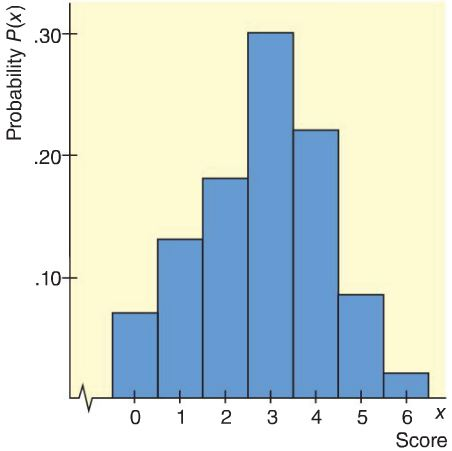
\includegraphics[width=3 in]{Image1.jpg}}
\end{frame}

\begin{frame}
\frametitle{Statistics and Probability Distributions}\pause
\begin{formula}
\begin{itemize}
\item The \textbf{mean} of a discrete population probability distribution is found by the formula
$$\mu=\sum X\cdot\Pr(X)$$\pause
\item The \textbf{standard deviation} of a discrete population distribution is found by the formula
$$\sigma=\sqrt{\sum(X-\mu)^2\Pr(X)}$$
\end{itemize}
\end{formula}\pause
\begin{definition}
The mean of a probability distribution is often called the \textbf{expected value} of the distribution.
\end{definition}
\end{frame}

\begin{frame}
\frametitle{Expected Value}\pause
\vspace*{-.15in}
\begin{example}
At a carnival, you pay \$2.00 to play a coin-flipping game with three fair coins.  You flip three coins at one time and you win \$1.00 for every head that appears.  Should your expect to win more money than you pay to play?
\end{example}\pause
\begin{itemize}
\item We begin by constructing the probability distribution for the number of heads.\pause
$$\begin{array}{|c|c|c|c|c|}
\hline
\text{\# of heads (X)}&0&1&2&3\\
\hline
\Pr(X)&\frac{1}{8}&\frac{3}{8}&\frac{3}{8}&\frac{1}{8}\\
\hline
\end{array}$$\pause
\item We now compute $X\cdot\Pr(X)$ for each value of $X$.\pause
$$0\cdot\Pr(0)=0\qquad\qquad 1\cdot\Pr(1)=\frac{3}{8}$$
$$2\cdot\Pr(2)=\frac{3}{4}\qquad\qquad 3\cdot\Pr(3)=\frac{3}{8}$$
\end{itemize}
\end{frame}

\begin{frame}
\frametitle{Expected Value}
\vspace*{-.15in}
\begin{example}
At a carnival, you pay \$2.00 to play a coin-flipping game with three fair coins.  You flip three coins at one time and you win \$1.00 for every head that appears.  Should your expect to win more money than you pay to play?
\end{example}
\begin{itemize}
\item We now compute $X\cdot\Pr(X)$ for each value of $X$.
$$0\cdot\Pr(0)=0\qquad\qquad 1\cdot\Pr(1)=\frac{3}{8}$$
$$2\cdot\Pr(2)=\frac{3}{4}\qquad\qquad 3\cdot\Pr(3)=\frac{3}{8}$$\pause
\item Using the formula for the mean of a probability distribution gives the expected value of 
$$0+\frac{3}{8}+\frac{3}{4}+\frac{3}{8}=\frac{3}{2}$$
\end{itemize}
\end{frame}

\begin{frame}
\frametitle{Expected Value}
\vspace*{-.15in}
\begin{example}
At a carnival, you pay \$2.00 to play a coin-flipping game with three fair coins.  You flip three coins at one time and you win \$1.00 for every head that appears.  Should your expect to win more money than you pay to play?
\end{example}
\begin{itemize}
\item Using the formula for the mean of a probability distribution gives the expected value of 
$$0+\frac{3}{8}+\frac{3}{4}+\frac{3}{8}=\frac{3}{2}$$\pause
\item Since you earn \$1.00 for each heads, you should expect to win an average of \$1.50 per game.  Since the game costs \$2.00 to play, you should expect a net loss of \$0.50 per game.
\end{itemize}
\end{frame}

\begin{frame}
\frametitle{Binomial Experiments}\pause
\begin{definition}
A \textbf{binomial experiment} is an experiment satisfying the following four conditions:
\begin{itemize}
\item There is a fixed number of trials, denoted $n$.\pause
\item The $n$ trials are independent and repeated under identical conditions.\pause
\item There are exactly two possible outcomes for each trial.  These outcomes can be considered \emph{success} and \emph{failure}.\pause
\item For each trial, the probability of success is the same.  We denote the probability of success by $p$ and the probability of failure by $q$.  Because each trial results in either success or failure, $p+q=1$. 
\end{itemize}\pause
The central problem of a binomial experiment is to find the probability of $r$ successes out of $n$ trials.
\end{definition}
\end{frame}

\begin{frame}
\frametitle{Binomial Experiments}\pause
\begin{example}
Determine if the following experiment  is a binomial experiment.  If it is not a binomial experiment, explain why.
\begin{itemize}
\item Selecting 20 university students and recording their class rank.
\end{itemize}
\end{example}\pause
This is not a binomial experiment because there are more than two outcomes for the variable.
\vspace*{3in}
\end{frame}

\begin{frame}
\frametitle{Binomial Experiments}
\begin{example}
Determine if the following experiment  is a binomial experiment.  If it is not a binomial experiment, explain why.
\begin{itemize}
\item Selecting 20 university students and recording whether they are on the Dean's list.
\end{itemize}
\end{example}\pause
This is a binomial experiment.
\vspace*{3in}
\end{frame}

\begin{frame}
\frametitle{Binomial Experiments}
\begin{example}
Determine if the following experiment  is a binomial experiment.  If it is not a binomial experiment, explain why.
\begin{itemize}
\item Drawing five cards from a standard deck of cards without replacement and recording whether they are red or black.
\end{itemize}
\end{example}\pause
This is not a binomial experiment because the probability of success will change with each draw.
\vspace*{3in}
\end{frame}

\begin{frame}
\frametitle{Binomial Experiments}\pause
\begin{example}
A survey from Teenage Research Unlimited found that $30 \%$ of
teenage consumers receive their spending money from part-time jobs.
We select 10 teenagers at random to determine the probability that exactly 4 of them will have part-time jobs.  Find the values $p,q,n,$ and $r$.
\end{example}\pause
\begin{itemize}
\item We will consider having a part-time job a success.\pause
\item Since $p$ is the probability of success, the example states that $p=0.3$.\pause
\item We can compute $q=1-p=0.7$.  Recall that $q$ is the probability of failure.\pause
\item We consider each selected teenager a trial.  So $n=10$.\pause
\item Since we want to consider the probability that exactly 4 of the selected teenagers will have a part-time job, $r=4$.
\end{itemize}
\end{frame}

\begin{frame}
\frametitle{Binomial Probability Distribution Formula}\pause
%\begin{formula}
In a binomial experiment, the probability of $r$ successes out of $n$ trials is given by the formula
$$\Pr(r)=\frac{n!}{r!(n-r)!}p^r\cdot q^{n-r}=(C_{n,r})\cdot p^r\cdot q^{n-r}$$
where $p$ is the probability of success in each trial and $q$ is the probability of failure in each trial.
%\end{formula}
\end{frame}

\begin{frame}
\frametitle{Binomial Probability Distribution Formula}\pause
\begin{example}
A survey from Teenage Research Unlimited found that $30 \%$ of
teenage consumers receive their spending money from part-time jobs.
If we select 10 teenagers at random, what is the probability that exactly 4 of them will have part-time jobs?
\end{example}
\begin{itemize}
\item In the previous example we found the following values
$$p=0.3\qquad\qquad\qquad q=0.7$$
$$n=10\qquad\qquad\qquad r=4$$\pause
\vspace*{-.1in}
\item Using the binomial probability distribution formula
$$\begin{array}{rcl}
\displaystyle \Pr(4)
&=&\displaystyle\frac{10!}{4!(10-4)!}(0.3)^4(0.7)^{10-4}\\ \\
&\approx&\displaystyle 0.2
\end{array}$$
\end{itemize}
\end{frame}

\begin{frame}
\frametitle{Binomial Probability Distribution Formula}\pause
\begin{example}
If a die is rolled 20 times, what is the probability that exactly half of the rolls will land on 3?
\end{example}\pause
\begin{itemize}
\item We begin by noticing that this is a binomial experiment.  Although there are six possible values on the die, we consider landing on a 3 a success and anything else a failure.\pause
\item Next we identify $n=20$, $r=10$, $p=1/6$ and $q=5/6$.\pause
\item Using the binomial probability distribution formula
$$\begin{array}{rcl}
\displaystyle \Pr(\text{Ten 3s})
&=&\displaystyle\frac{20!}{10!(20-10)!}\left(\frac{1}{6}\right)^{10}\cdot\left(\frac{5}{6}\right)^{20-10}\\ \\ \pause
&\approx&0.00049
\end{array}$$
\end{itemize}
\end{frame}

\begin{frame}
\frametitle{Mean and Standard Deviation}\pause
%\begin{formula}
In a binomial experiment
\begin{itemize}
\item $\mu=np$
\item $\sigma=\sqrt{npq}.$\pause
\end{itemize}
The mean value $\mu$ can be thought of as the \textbf{expected number of successes} in the experiment.
%\end{formula}\pause
\begin{example}
If we roll a single die 20 times, how many times can we expect 3 to roll?
\end{example}\pause
\begin{itemize}
\item Using the binomial experiment formula for $\mu$, we can expect the number of 3s rolled to be 
$$\mu=20\cdot\left(\frac{1}{6}\right)=3.\overline{3}$$
\end{itemize}
\end{frame}

\begin{frame}
\frametitle{Mean and Standard Deviation}
%\begin{formula}
In a binomial experiment
\begin{itemize}
\item $\mu=np$
\item $\sigma=\sqrt{npq}.$
\end{itemize}
The mean value $\mu$ can be thought of as the \textbf{expected number of successes} in the experiment.
%\end{formula}
\begin{example}
If we roll a single die 20 times, how many times can we expect 3 to roll?  Find the standard deviation for the number of 3s rolled.
\end{example}\pause
\begin{itemize}
\item Using the binomial experiment formula for $\sigma$, find the standard deviation for the number of 3s rolled to be
$$\sigma=\sqrt{20\cdot\left(\frac{1}{6}\right)\cdot\left(\frac{5}{6}\right)}=1.\overline{6}$$
\end{itemize}
\end{frame}

\end{document}
